\documentclass{article}
\usepackage[utf8]{inputenc}
\usepackage[T1]{fontenc}
\usepackage{geometry}
\usepackage{graphicx}

\geometry{margin=0.5in}

\begin{document}

\section*{Task}
You need to write and run a program that measures a person's reaction time to a randomly appearing light signal. \underline{The program should be implemented using interrupts and should operate independently of the main program.} \\

\subsection*{\underline{Task's criteria}}
\begin{itemize}
    \item you must use two buttons
    \begin{itemize}
        \item P4.0 (STOP) - pressed in response to the start signal of the measurement
        \item P4.1 (INIT) - initiates the measurement sequence
    \end{itemize}
    \item measurement accuracy: 0.01 seconds
    \item maximum measurement time: 1 second
    \item random wait time for the start signal between 1 and 6 seconds with a resolution of 0.01 seconds
    \item after pressing INIT, the displays turn off
    \item the start signal for the measurement is the display of the number \textquoteleft\textbf{00}\textquoteright
    \item STOP stops the measurement
    \item the measurement result (\textbf{XX}) is displayed until INIT is pressed again
    \item button handling may (but does not have to) be implemented in the P1 interrupt\textsuperscript{*)}
\end{itemize}

\noindent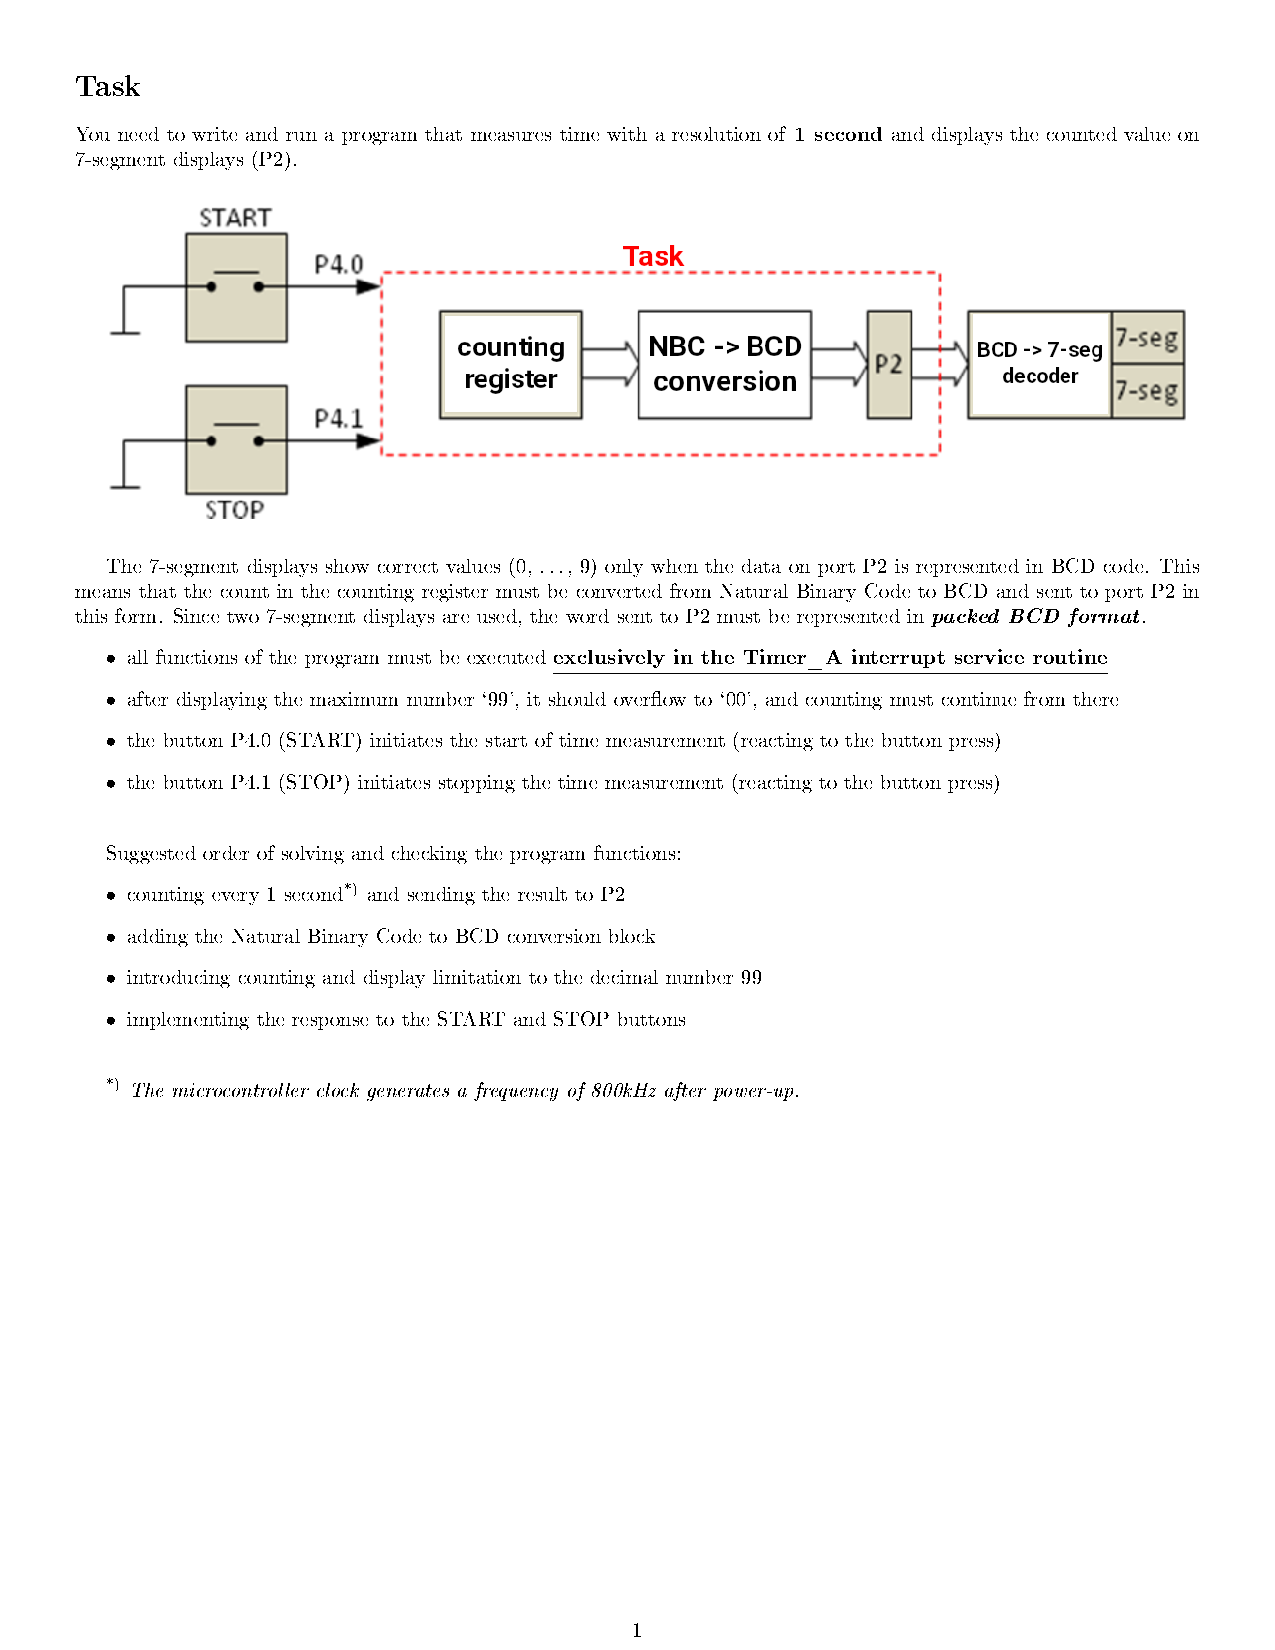
\includegraphics[width=\textwidth]{"img/TIMER_A_NBC2BCD_2.png"}
\vspace{5mm}

\textsuperscript{*)} \textit{The connection diagram explaining the connection of buttons (P4) with port P1 is presented in the document \\ "Blocks\_scheme.pdf" (block 7).}

\end{document}